\documentclass{article}
\usepackage[utf8]{inputenc}
\usepackage{hyperref}
\title{Implementation Details and Design of DPDK based RAN-emulator}
\author{Prateek Agarwal}
\date{May 2021}

\usepackage{graphicx}
\graphicspath{ {./} }

\begin{document}

\maketitle
\tableofcontents

\section{Introduction} \label{Intro}
This document explains the implementation details of DPDK based RAN-emulator. The main purpose of this report is to ensure that any future developer can understand RAN code and should be able to further modify or extend it as per requirement.

This network function acts as the load generator for the testing of user plane forwarding function.
The load needs to be generated in various modes for the testing of UPF forwarding capabilities.
Section \ref{tools} suggests some of the tools that should be learnt to handle large code base easily and be productive while doing so.

\section{Tools} \label{tools}
Learn the tools mentioned in this document.
Some of them are necessarily required to move through a large code base such as the 5G test bed project. Others are strongly advised to increase your productivity and save you a whole lot of time.
\subsection{Visual Studio Code}
Please use Visual Studio code to read/write code. Vscode is an excellent and a  basic IDE for writing C/C++ code. Most of us use vscode for our development work. The use of vscode will help in better communication with the team members. Here are some of the important features that we routinely use:
\begin{itemize}
    \item \textbf{Remote SSH} You can login remotely to the server from the editor itself. This implies that you do not need GUI applications like team-viewer etc. to use an editor or login on a graphical interface. These applications are heavy and affects your overall productivity and development experience.
    \item \textbf{Refactoring, Formatting etc. Shortcuts} See what F2, F12, Shift + F12, ctrl + shift + I are used for. You will find them very useful.
    \item \textbf{Terminal Support} Terminal support is available inside the editor. I have frequently used for building the executable after making some changes and while working on further changes simultaneously.
\end{itemize}
\subsection{Vim}
This is not necessarily required but strongly advised. If you learn vim (which has initial steeper learning curve), you will thank me later.
This point may look contradictory to the first point. But it is not. You \textbf{must} use Vim key bindings in Vscode.
Resources:
\begin{itemize}
    \item A nice place to get started is \url{https://www.youtube.com/watch?v=a6Q8Na575qc&t=2s} .
    \item Practice multiple times on terminal with the help of \textbf{vimtutor}.
\end{itemize}
\subsection{SSH keys}

Install SSH key on the remote server as soon as possible for smoother login into the remote machine. Keys if installed do not require you to type password again and again and will save you from a lot of unnecessary repeated work. When the key is installed on the remote machine, the server identifies your machine. Use aliases or scripts to login through SSH.

\subsection{Git}
It is required. Learn it properly from experts, review it multiple times. Learn the internal working of Git rather than copying commands from stack overflow without understanding what they mean. There is no other alternative.
Inadequate knowledge of git version control system can create a lot of stress for you and nuisance for others. Do not push commits on other person's branch . Keep updating the gitginore file so as not to push binary executables or other files not meant to be pushed on the remote repo.
\begin{itemize}
    \item \textbf{Important Commands}: Add, reset, commit, branch, merge (three-way and ff), difference between pull and fetch, git log, stash. Vscode is good for handling merge conflicts as well. Learn how to write gitginore.
    \item \textbf{Book} \url{https://git-scm.com/book/en/v2} Chapter 1,2,3 are compulsory reading.
          Read other chapters if you are interested or feel the need. Review them periodically.
    \item \textbf{Video} There are many good videos on the web with hardly any difference in the quality. Some of them are so basic that you lose interest midway. \url{https://www.youtube.com/watch?v=2sjqTHE0zok&t=3s} is one of the videos that suits the M.Tech second year students at IIT Bombay.
\end{itemize}
\subsection{Terminal Multiplexers}
Learn how to use tmux or screen for command line. You will find terminal multiplexers useful while running multiple network functions on the same host and connecting to the multiple servers simultaneously.

I use tmux. It is also good for pair programming. tmuxinator can be used to make config files for saving the session configurations. The .tmux.conf file on turing 4, turing 5 has all the configurations one need. Kindly understand these config files. See the tmuxinator configurations in ~/.config/tmuxinator on turing 5 to learn how to write tmuxinator configurations.

Resources:
\begin{itemize}
    \item The snippets/ideas for configuration files are drawn from \url{https://www.amazon.in/tmux-2-Brian-P-Hogan/dp/1680502212/ref=sr_1_1?dchild=1&keywords=tmux&qid=1619933598&sr=8-1}
    \item See the MIT missing semester video lecture on tmux.
\end{itemize}
\subsection{Important bash utilities/commands}
\begin{itemize}
    \item \textbf{grep} Know the flags. Useful flags : -i, -n, -r, -l , -A, -B , -C .
    \item \textbf{cut} This command is very useful for dissecting the log files for the cleaning of data. Flags: -d, -f
    \item{Other useful commands} Ctrl-R, less, cat, sudo !!, history, !$<$command number in history$>$  etc.
    \item Please do \textbf{NOT} use sudo for everything. It is a poor practice on a multi user system and is against the principle of least privilege. Many students do this and keep doing this for the entire year. It messes up file permissions besides being disaster prone.
\end{itemize}
\subsection{Debugging}
\begin{itemize}
    \item \textbf{GDB}
I found gdb to be very useful in debugging segmentation faults. It is good to have a hands on practice on gdb with the help of a cheat sheet available online. Although \textbf{bt} or \textbf{backtrace} command is all you need for handling segmentation faults.

Resources: Cheatsheet \url{http://csapp.cs.cmu.edu/3e/docs/gdbnotes-x86-64.pdf}
\item \textbf{Log files} The use of regex  inside vim or otherwise in searching logs. In particular, ASN Logs  for knowing amfUeNgapId and ranUeNgapId combinations.

Checking thread id and timestamp also forms an important part of debugging.

\end{itemize}
\subsection{C++}
C++ is not only C with STL. It is an ocean in itself to learn and I am still learning it. There are certain idioms and ways of the language which do not make sense but they are still there. Only relying on stack overflow like all of us do for python, bash and other scripting languages will not work here. I am listing down some ideas which will be helpful and will save you a lot of time with C++.
\begin{itemize}
    \item \textbf{extern C directive} - This helps in keeping both C and C++ code in the same source code and must be used while including C only headers. This is  required in using some of the DPDK headers. Otherwise you may get undefined reference error.
    \item Avoid \textbf{using namespace std;} and other such directives in writing the new code. This pollutes the namespace and creates confusion for other developers. I did not remove this until now as this is deeply entrenched and used multiple times in headers/source files.
    \item Use \textbf{auto} keyword wherever you can. Using auto is enough as the type can be inferred during compilation.
    \item Other items may be added as required.
\end{itemize}


\section{Core Layout}
NUMA- node 1 with starting core 12 is currently used by the RAN.
\begin{itemize}
    \item \textbf{CORE\_RX\_POLL}: Receives all the incoming packets from UPF. These includes the latency packets or data packets in the downlink direction.
    \item \textbf{CORE\_TX\_START - CORE\_TX\_END}
          These cores are used to send data packets in the uplink  direction i.e. from RAN to UPF.
    \item \textbf{CORE\_RTT}
          This core sends the data plane latency packets in the uplink direction. These packets are reflected back by the DNN so that end to end latency can be measured.
    \item \textbf{CORE\_CP\_TRAFFIC} This core sends the control plane traffic. A separate core was used so that a call back can be registered for storing timestamps. These timestamps are used for calculating control plane latency.
    \item \textbf{CORE\_MISC and CORE\_STAT}
          These cores handles miscellaneous functions like ARP handling, timer and logging of stats.
\end{itemize}
Using this layout, a maximum of 7 cores are available for the data forwarding on the same numa node. To increase this number, the functions running on CORE\_MISC and CORE\_STAT can be run parallely on the same core.  




\section{Modes of Operation}
The load generator can be used in different modes to characterize the different behaviors of the user plane function. The various modes are
\begin{itemize}
    \item Setup Sessions and Send Data.
    \item Send only control plane traffic.
    \item Send Control Plane and Data Plane traffic simultaneously.
    \item Helper functions.
    \item QoS functions.
\end{itemize}
\subsection{Setup sessions and send data}
Initially sessions are setup by sending session establishment and session modification messages directly from the RAN to the UPF.
Once the sessions are setup the data packets are forwarded from CORE\_TX\_START- CORE\_TX\_END (inclusive). 
Control plane latency is calculated during the initial setup for all the session related packets. Throughput is also logged in the log file.
The number of UEs/sessions that are used for sending data per core is asked to the user. The sessions are partitioned in disjoint sets among the cores before forwarding.

\subsection{Send only control plane traffic}
This mode is used to send only control plane traffic and no data plane forwarding takes place.
This is a synthetic traffic i.e. it does not represent any real world scenario. The main motive behind this mode was to saturate control plane and measure control plane handling capabilities of the different designs of the UPF. The latency and throughput values are logged in the file as earlier.
This is an open load test in which session establishment, release and modification packets are sent one by one with a user provided inter packet delay (in us). These packets are sent from CORE\_CP\_TRAFFIC. The open load means that the RAN does not wait for response packets before sending
 the next packet.  Ideally modification message should be sent only once the session establishment response is received. However, open load is a good approximation of the actual behavior and is easy to implement.
 
\subsection{Send Control Plane and Data Plane Traffic Simultaneously}
$n1$ sessions are established before the data forwarding takes place. These sessions remain established throughout the run.
$n2$ sessions are established, modified and released while the data forwarding is also taking place. The data packets are sent from all the currently established sessions. The minimum value of currently established sessions is $n1$. The maximum value is $n1+n2$.
The duration $t1$ for which all the static sessions $n1$ and the dynamic sessions $n2$ are used is also asked to the user. 

So $n2$ sessions are established, modified and then after waiting for the time $t1$, the $n2$ sessions are released. This establishment, modification and release cycle continues for the entire duration of the experiment.
Each of the data packet forwarding cores use all the existing established sessions/UEs to forward the data. Note that this is different from the case when sessions were partitioned among cores.
\subsection{Helper Functions}
There is only one helper function right now. This helper function - Delay Estimator - helps in mapping inter batch delay with the data forwarding throughput of the load generator for a given number of cores and sessions. 
This mapping is used to set the rate of forwarding of the data packets. Intel 40Gbps NICs that we have does not have rate limiting APIs like 10Gbps NIC.

\subsection{QoS Functions}
These functions were developed to check the correctness of QoS algorithms deployed at the UPFs. These functions were tested on 10Gbps NIC systems and may require modification for other NICs.


For QoS testing, it was required to test whether the packet forwarding rate is actually limited by
 the algorithm. For this, data is forwarded at a low rate and at a high rate. The low rate is lower than  the rate limit imposed on the sessions. The high rate is higher than the limit. So when the rate is higher, the output at UPF is limited to the rate limit. 
 
 Lower rate - 700 Mbps, High rate - 1200 Mbps, Rate limit -1000 Mbps. When the incoming rate at the UPF is 1200 Mbps, outgoing rate is 1000 Mbps if the QoS algorithm is correct.

\section{Run Time Options}
\begin{itemize}
    \item The inter batch delay in microseconds. Larger the delay, slower the forwarding rate.
    \item Number of UEs per core. Per Core different UE count can be given by setting the macro ENABLE\_DIFF\_PER\_CORE\_UE\_COUNT to 1. This option was required for producing skewed traffic.
    \item Number of sessions that will be used for forwarding the data.
    \item \textbf{Type of payload}
          There are two available options:
          \begin{itemize}
              \item \textbf{Payload Size} Can be set to anything in the range 64-1400 bytes. The smaller payload size requires higher header processing per byte at UPF.
              \item \textbf{IMIX traffic} IMIX distribution resembles the real world traffic. The distribution mentioned on \url{https://en.wikipedia.org/wiki/Internet_Mix} is used to model IMIX traffic in out case.
          \end{itemize}
    \item \textbf{Interval to Switch Rates (t)} Interbatch delay is reduced in the step sizes provided by the user on input.
          After every interval t, step size is subtracted from the existing delay.
    \item   $n1$, $n2$, $t1$ are asked when the control plane and data plane traffic is sent simultaneously.
\item Data Plane latency options while forwarding are
\begin{itemize}
    \item\textbf{1} - Send latency packets from all the established sessions.
    \item\textbf{2} - Send latency packets from a specified session.
    \item\textbf{3} - Do not send data plane latency packets.
\end{itemize}
          These are explained in the corresponding modes of operation.

\end{itemize}

\section{Algorithms}
\subsection{Forwarding Algorithms}
\subsubsection{Data Plane}
Once the sessions are established, their contexts are stored in the vector \textbf{storedUeContext}. These contexts are used to
create data packet headers. Payload is same for all the packets. The entire raw packets are created before
the forwarding loop. Each session is used to send data in batches. Pre-computation of packets and batching
helps in sending data at high speed that is sufficient to saturate 40Gbps NIC.

\subsubsection{Control Plane}
In a 5G-conforming RAN, the session related messages are sent by SMF to UPF.
This RAN-emulator's primary role is that of a load generator. Session related messages - session establishment, modification and release messages are directly sent by RAN to the UPF.
There are however some functions defined before the start of the load testing mode in the main function that interacts with AMF and to SMF through AMF. These are not removed as they act as a stub for interaction with AMF. They can be deleted after rigorous testing.

The session establishment, modification and release packets have a standard format of the header as well as the
payload. These packets are defined as static arrays in the source file dpdk\_ran.cpp - pfcpSessionEstablishmentRequestPacket, pfcpSessionModificationRequestPacket and pfcpSessionReleaseRequestPacket.
Before sending these packets, the fields pertaining to a particular session are modified in these packets.
These fields include source IP, tunnel end point identifier (teid) and session ids.
There are counter variables defined in the dpdk class which maintain the next session related fields.
Examples include nextUEIPEstablishment, nextTEIdEstablishment etc. These counters are updated after packet is sent.
Only one control plane packet is sent at a time i.e. batch size is one.
\subsection{Latency Calculation Algorithms}
\subsubsection{Key Concept}
When packets are transmitted from RAN, the timestamp when the packet is forwarded is stored for the outgoing packet. When the response for the packet arrives at the receiving side of RAN, the difference in time values of the current time and the stored timestamp  is calculated and then reported in the log file.
\subsubsection{Storing of Timestamp}
\begin{itemize}
    \item \textbf{Data Plane} The packet identification field in the IP header is used to identify the packet. These latency packets
          are sent from the core CORE\_RTT. All the established sessions/UEs are used for forwarding the traffic. When the packet is
          transmitted, a callback  function stores the outgoing packet timestamp in a hashmap with packet id as the key. This field is
          generally used in the fragmentation and reassembly of packet data. The data plane latency packet throughput is substantially reduced by introducing sleep commands. The option of disabling the calculation of latency is removed as latency packets do not significantly affect any other metrics. Data plane latency is independently logged in a different column in the log file.
    \item \textbf{Control Plane}
          This requires deep packet inspection of control plane packets. These packets are sent from the core CORE\_CP\_TRAFFIC.
          There are three types of control plane packets - session establishment, session modification and session release packets - all of
          them are used for measuring control plane latency. These packets have session ids stored at different offsets in the payload. A
          hashmap is maintained in which the key (64 bits length) is composed of :
          \begin{itemize}
              \item 16 MSB bits store the message type i.e. establishment (50), modification (52), and release (54).
              \item The next 48 bits store the session ids.
          \end{itemize}
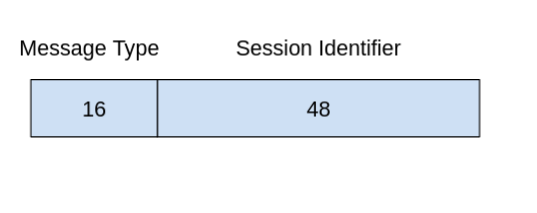
\includegraphics[width=0.6\textwidth]{KeyField.png}


          A callback function is registered on  the transmit queue corresponding to CORE\_CP\_TRAFFIC which stores the timestamp in the hashmap.
\end{itemize}
\subsubsection{Calculation of Latency}
A single callback function is registered on the CORE\_RX\_POLL which  receives the incoming packet.
\begin{itemize}
    \item \textbf{Data Plane} The same outgoing packet is reflected by the DNN packet and stored timestamp is retrieved from the hashmap and the difference is the end to end latency of each packet.
    \item \textbf{Control Plane} Every control plane packet has a response packet - establishment response (51), modification response (53), release response (55). The control plane latency is the time period from when the request packet is sent and the response packet is received.
          The response packets have message type and either session IDs in their payload. For modification and deletion  responses, the session ids have a difference of 3000. So the key is retrieved from the response packet and difference in the current time and the stored timestamp is calculated.
\end{itemize}
\subsubsection{Why do we need different techniques for control plane and data plane?}
\begin{itemize}
    \item \textbf{Why can't we use packet identifier for control plane packets?}
          Both types of packets are received on the same rx queue/core. So, only the packet identifier in ip header is not enough to differentiate control plane and data plane packets. And you will need deep packet inspection to differentiate among the two packets.
    \item \textbf{Why don't we inspect packet payload for data plane packets?} Data plane packet has no useful payload and when the ip header identification field is unused till now, we can use it.
          \item \textbf{Development Sequence}
          Data plane latency was implemented earlier when the packet id field was unused. Control plane latency calculation is done later.
\end{itemize}

\subsubsection{Callback functions}
Call back functions are registered on receive and transmit queues for latency calculation.
\begin{itemize}
    \item \textbf{dataPlaneStoreTimestampCallback}
          This callback is registered on CORE\_RTT for storing the timestamp of outgoing  data plane latency packets.
    \item \textbf{controlPlaneStoreTimestampCallback} This callback is registered on CORE\_CP\_TRAFFIC for storing the timestamp of outgoing control plane packets.
    \item \textbf{calculateLatencyCallback} This callback is registered on CORE\_RX\_POLL for inspecting the incoming packets.
          These packets are either response packets to control plane packets or the data plane packets reflected back by DNN. The difference in the current time and the timestamp stored during the tx callbacks gives the latency values.
\end{itemize}
\section {Files and Folders}
DPDK\_RAN folder is created inside the 5GCore folder. This folder hosts all the relevant code, headers, build and log files.
This section describes the relevant files that are present in this folder.
\begin{itemize}
    \item \textbf{loadDPDK.sh} This script creates the dpdk binaries in the utility/dpdk/x86\_64-linuxapp-gcc folder.
          This script also asks for the PCI addresses of the NIC ports that will be used by the DPDK Application.
          The generation of Makefile using CMake and the build using make is also performed by this script. This script is required to be
          run only once after every reboot. The ports need to be unbind from kernel driver before executing this script. Use make to rebuild after every source code/ header modification.
    \item \textbf{CMakeLists.txt} This file is used by CMake to generate make files. Going through this file will help in understanding various dependencies. Writing a new CMakeLists.txt may require the study of documentation present on their webpage.
    \item \textbf{include/}
          \begin{itemize}
              \item \textbf{include/dpdk\_config.h}
                    This header has various options which are used to change the code cofiguration before the compilation of the source.
                    \begin{itemize}
                        \item \textbf{NUM\_TX\_CORE} - Number of Data Forwarding Cores.
                        \item \textbf{RATE\_LIMITER} - This is used to determine the data forwarding rates. Different options are explained in the header file itself. Frequestly used option is 5.
                        \item \textbf{ENABLE\_GTP\_EXTN\_HEADER} : This option enables/disables the GTP Extension header. RTC model that uses customized hash function which parses the inner GTP headers requires extension headers to be disabled. For other models, kindly \textbf{enable} GTP extenstion header.
                        \item \textbf{USE\_CUSTOM\_UE\_IP\_SEQ} 
                        Source IP sequence is drawn from the file misc\_ds.h rather than being generated during the run.                        
                        
                        \textbf{Usage} :This option is useful in sending skewed traffic in Run-to-Completion Model. The
                              mapping of source UE IPs to the corresponding UPF core are generated before the run. This mapping is used to populate
                              the custom IP sequence vector in the misc\_ds.h. For example, if I want to send high traffic directed at a single UPF
                              core, say core with the index 0. I would like to send traffic from a total of 200 sessions. Two forwarding cores at
                              the RAN can be used to forward traffic by distributing sessions as 25,25,75,75 respectively on the four cores. First
                              50 sessions in the misc\_ds.h vector should map to the core with 0 index in such a case.
                    \end{itemize}
              \item \textbf{include/dpdk\_ran.h}
                    This header has the declaration of the class dpdk. This class is a singleton class which has almost all of the useful functions
                    and variables declared. This also has definitions of the structures like PDI and PDR. Most of the new development will require the
                    understanding and modification of this header.
              \item \textbf{include/ranMain.h} The earlier implementation had declared and defined all the  procedures in the source file
                    ranMain.cpp. This file was 10000 lines of code and it was difficult to understand and modify it. There was a lot of dead code
                    which was never called. To make life simple, the source was bifurcated into two files ranMain.cpp and ran.cpp. This header is common to both the source files and contains the declarations of all the procedures in ran.cpp.

              \item \textbf{include/misc\_ds.h} This file contains two important parameters.
                    \begin{itemize}
                        \item \textbf{Delay Sequence} This is a two dimensional vector in which each row contains the delay sequence for a data forwarding core. This delay sequence is obtained using the delay estimator helper function.
                        \item \textbf{Custom UE IP sequence} Explained in its usage in dpdk\_config.h (the previous point).
                    \end{itemize}

              \item \textbf{include/test\_ue.h} This header contains ue context related structure definition. You may not need to touch this header for running experiments.

          \end{itemize}
          \item \textbf{src/}
          \begin{itemize}
    \item \textbf{src/ranMain.cpp}
          This file contains the main routine.
    \item \textbf{src/ran.cpp} This file contains:
          \begin{itemize}
              \item  All the procedures that are called by main routine.
              \item  This file also has some other procedures/methods which could have been defined as a part of the dpdk class itself.
              \item Some procedures that are called by dpdk APIs are required to be defined either as a static member of the class or within the same translation unit i.e. same source file.
          \end{itemize}

    \item \textbf{src/dpdk\_ran.cpp}
          This file contains the functions that are a part of the dpdk class and can be divided according to their functionality as follows:
          \begin{itemize}
              \item Callback Functions
              \item \textbf{Packet forwarding functions} These include the sub routines that are called by the procedures corresponding to different modes. Example: sendUDPdata is called by different modes for packet forwarding.
              \item Logging and displaying of statistics.
              \item Other functions which may not require subsequent modification.
          \end{itemize}

    \item \textbf{src/dpdk\_config.cpp}
          This is the config file that initializes and sets up the dpdk. These may require configuring ports, queues, offloads. Most of the code here is drawn from standard DPDK applications like testpmd. These may not require modifications unless there is a complete overhaul.
        \end{itemize}
    \item \textbf{log/}
    \begin{itemize}
        \item \textbf{throughput/} This folder contains all the generated data measurement files. These files contains throughput and latency values measured during the run.
        \item \textbf{dpdk\_ran/} This folder contains all the logs generated during the run. These files contain logging data according to the level of logging set during the compilation. 
    \end{itemize}
\end{itemize}
\section{DPDK APIs used}
List of all DPDK APIs with their description, list of arguments and the return value is available at \url{https://doc.dpdk.org/api/index.html}. Although the list on documentation is according to the latest version of DPDK, function signatures do not change across implementations. There is a deprecated functions list on the documentation page to check for the list of deprecated functions. This implies that do not be hesitant in looking at the documentation on the webpage irrespective of the version mismatch. The only issue with the documentation is that its search functionality is not upto the mark. It does not account for spelling mistakes etc. Moreover searching on google for DPDK APIs is also not very effective.
I shall list down the most frequently used APIs and what I think any new developer who extends the code needs to know. Kindly refer to  the documentation on the url for correct use and complete understanding.
\begin{itemize}
    \item rte\_eal\_remote\_launch,rte\_eal\_wait\_lcore
    \item rte\_pktmbuf\_mtod\_offset
    \item rte\_eth\_tx\_prepare, rte\_rth\_rx\_burst
    \item rte\_be\_to\_cpu\_(64, 32, 16)
    \item rte\_eth\_add\_(tx,rx)\_callback
    \item rte\_delay\_(ms,us), rte\_rdtsc, rte\_timer\_init, rte\_get\_timer\_hz, rte\_get\_timer\_cycles
    \item struct rte\_(ipv4,udp)\_hdr
    \item rte\_lcore\_id, rte\_lcore\_count
    \item rte\_mempool\_get\_bulk, rte\_pktmbuf\_reset\_headroom
\end{itemize}
\end{document}
